% ---------------------------------------------------------------- 6 results
\section{Results and Discussion}
\label{sec:results}

\subsection{Link-level operating point on the base corpus}
\label{sec:results-base}

Table~\ref{tab:base} gives the free-running token accuracy and BLEU-4 of the codec on 200 test sentences of the base corpus over AWGN at 10\,dB, for four receiver priors and a greedy decoder. The language prior lowers the rate needed for a given fidelity at every prefix length: at 6 symbols per token GPT-2 decides 85.7\,\% of the tokens correctly, against 73.7\,\% with token frequencies alone and 70.3\,\% with no prior, and BLEU-4 rises from 0.38 (no prior) to 0.71. The last row is a diagnostic that gives the receiver the true preceding sentences of the document and bounds what the fast memory can contribute (89.3\,\% at 6 symbols). Under Rayleigh block fading at 10\,dB and 8 symbols per token the four priors reach 0.681 (none), 0.731 (unigram), 0.758 (GPT-2) and 0.785 (GPT-2 with true history). At 0\,dB the order reverses: GPT-2 falls below the unigram prior at every prefix length (0.119 against 0.196 at 8 symbols per token), most likely because the greedy decoder then follows its own early errors. The operating point of this study is therefore an SNR around 10\,dB.

\begin{table}[t]
\centering
\caption{Free-running token accuracy and BLEU-4 on the base corpus (200 test sentences, AWGN, 10\,dB, greedy decoding) for four receiver priors, against the number of real channel symbols per token $m$.}
\label{tab:base}
\small
\begin{tabular}{@{}lcccccccc@{}}
\toprule
 & \multicolumn{4}{c}{Token accuracy} & \multicolumn{4}{c}{BLEU-4} \\
\cmidrule(lr){2-5}\cmidrule(l){6-9}
Receiver prior & $m=4$ & $m=6$ & $m=8$ & $m=12$ & $m=4$ & $m=6$ & $m=8$ & $m=12$ \\
\midrule
None (maximum likelihood) & 0.3728 & 0.7032 & 0.9119 & 0.9980 & 0.0354 & 0.3813 & 0.7672 & 0.9946 \\
Unigram & 0.4081 & 0.7366 & 0.9291 & 0.9985 & 0.0506 & 0.4261 & 0.8152 & 0.9971 \\
GPT-2 & 0.4633 & 0.8570 & 0.9706 & 0.9995 & 0.1839 & 0.7059 & 0.9273 & 0.9990 \\
GPT-2 + true history (diagnostic) & 0.5510 & 0.8930 & 0.9818 & 0.9995 & 0.3103 & 0.7819 & 0.9607 & 0.9990 \\
\bottomrule
\end{tabular}
\end{table}

Rate nesting costs nothing measurable at the prefix that was checked: a codebook trained with the same budget for 8 symbols per token only reaches a channel-only token accuracy of 0.8890 at 10\,dB on 2000 held-out tokens, and the nested codebook, read at its 8-symbol prefix, reaches 0.8885. Other prefix lengths were not tested. Before block power control, the codewords of the base corpus have an average power of 0.81--0.89 per symbol over the six prefixes; block power control raises every transmitted block to exactly one.

\subsection{Decoder of selective refinement}
\label{sec:results-decoder}

Table~\ref{tab:decoder} reports the selection on validation text. In stage~1, a first round of 4 symbols has the lowest criterion (8.652 symbols per token), and a first round of 6 symbols (8.730) is within 1\,\% of it and needs fewer rounds (3.01 against 4.01 per message), so it wins under the rule. Reopening loses in every case: it decodes more accurately for the same forward symbols, but every token with shells left must then take part in every round's decision, and that signalling costs more than it saves. In stage~2, beam search of width 4 lowers the criterion by 4.9\,\%, above the 2\,\% bar, whereas width 2 (1.5\,\%) does not. The selected decoder---beam width 4, a first round of 6 symbols, no reopening---needs 7.4\,\% fewer symbols than the greedy decoder from 2 symbols. The selection also shows that beam search helps the fixed prefix far more than it helps refinement: with width 4 the fixed prefix needs 17.7\,\% fewer symbols than with greedy decoding (9.049 against 10.994), because the beam removes much of the error propagation that refinement had been compensating for. Every fixed-prefix reference below is decoded with the same beam, so the comparisons are made against this stronger baseline.

\begin{table}[t]
\centering
\caption{Selection of the decoder on validation text (96 messages, 1633 tokens, mean SNR 9.8\,dB): real channel symbols per token for 90\,\% token accuracy, decoded for real. Selective refinement is charged its signalling at the entropy (criterion) or as a bitmap; the fixed prefix is decoded with the same beam width. Rounds per message at confidence 0.95.}
\label{tab:decoder}
\small
\begin{tabular}{@{}cccccccc@{}}
\toprule
Beam & \makecell{First round\\(symbols)} & Reopening & \makecell{Forward\\only} & \makecell{+ signalling\\(entropy)} & \makecell{+ signalling\\(bitmap)} & \makecell{Fixed prefix,\\same beam} & \makecell{Rounds per\\message} \\
\midrule
1 & 2 & no  & 7.527 & 8.971 & 9.442  & 10.994 & 5.00 \\
1 & 2 & yes & 7.486 & 9.937 & 10.541 & 10.994 & 5.34 \\
1 & 4 & no  & 7.395 & 8.652 & 8.740  & 10.994 & 4.01 \\
1 & 4 & yes & 7.682 & 9.640 & 10.060 & 10.994 & 4.22 \\
1 & 6 & no  & 7.836 & 8.730 & 8.758  & 10.994 & 3.01 \\
1 & 6 & yes & 8.211 & 9.533 & 9.948  & 10.994 & 3.20 \\
2 & 6 & no  & 7.738 & 8.603 & 8.637  & 10.044 & 3.01 \\
\textbf{4} & \textbf{6} & \textbf{no} & \textbf{7.492} & \textbf{8.306} & \textbf{8.357} & \textbf{9.049} & \textbf{3.01} \\
\bottomrule
\end{tabular}
\end{table}

\subsection{Primary endpoint on the drift stream}
\label{sec:results-primary}

Table~\ref{tab:primary} and Figure~\ref{fig:primary} give the primary endpoint. With its memories and selective refinement, DN-SC reaches 90\,\% token accuracy with 7.08 real channel symbols per token, against 9.23 for the frozen fixed-rate receiver: a saving of 23.3\,\% with the return-link signalling charged at its entropy (28.3\,\% for the forward symbols alone and 20.7\,\% with an explicit bitmap). The saving is observed on every seed, between 10.5\,\% and 28.5\,\% ($p = 0.031$, the smallest value six seeds allow), and on the three seeds that had never been run before (20.6\,\%). Decoded for real on the audited steps, the saving is 27.9\,\% (95\,\% CI 21.6--31.7\,\%; 26.3\,\% with a bitmap), again on every seed (Holm-adjusted $p = 0.094$), and 25.9\,\% (95\,\% CI 11.0--33.2\,\%) on the unseen seeds alone. Seed~3 is the weakest on both measures ($-10.5$\,\% teacher-forced, $-9.1$\,\% decoded for real). These figures do not include the synchronisation of the shipped memories, which is charged separately in Section~\ref{sec:results-crossover}.

\begin{table}[t]
\centering
\caption{Real channel symbols per token for 90\,\% token accuracy on the hierarchical drift stream (GPT-2 prior, beam-4 decoder for every receiver). Selective refinement includes its return-link signalling at the entropy; synchronisation is not included. Teacher-forced: mean over seeds, all 600 steps. Decoded for real: 26 audited steps per seed, curves pooled over the seeds, 95\,\% paired bootstrap interval in brackets. Changes are relative to the frozen fixed-rate receiver on the same seeds.}
\label{tab:primary}
\small
\begin{tabular}{@{}lcccccc@{}}
\toprule
Receiver & Seeds & \makecell{Teacher-\\forced} & Change & \makecell{Decoded\\for real} & Change [95\,\% CI] & $p$ \\
\midrule
Frozen, fixed rate & 6 & 9.23 & --- & 10.37 & --- & --- \\
Frozen + refinement & 6 & 7.80 & $-15.4$\,\% & 8.36 & $-19.3$\,\% [$-21.4$, $-15.6$] & 0.031 \\
Context memory, fixed rate & 4 & 8.04 & $-10.1$\,\% & 9.05 & $-10.6$\,\% [$-16.1$, $-5.3$] & --- \\
Context memory + refinement & 4 & 7.18 & $-19.8$\,\% & 7.55 & $-25.4$\,\% [$-29.0$, $-15.6$] & 0.125 \\
DN-SC memories, fixed rate & 6 & 7.80 & $-15.5$\,\% & 8.17 & $-21.2$\,\% [$-23.9$, $-14.9$] & --- \\
\textbf{DN-SC + refinement} & 6 & \textbf{7.08} & $\mathbf{-23.3}$\,\% & \textbf{7.48} & $\mathbf{-27.9}$\,\% [$-31.7$, $-21.6$] & 0.031 \\
\bottomrule
\end{tabular}
\par\smallskip
\begin{minipage}{0.97\linewidth}\footnotesize
$p$: exact sign-flip test on the per-seed costs decoded for real (refinement receivers against the frozen fixed-rate receiver); Holm-adjusted 0.094, 0.125 and 0.094 for the three rows. Per-seed changes of DN-SC + refinement, seeds 0--5: $-23.0$, $-26.1$, $-28.2$, $-10.5$, $-20.0$, $-28.5$\,\% (teacher-forced) and $-27.9$, $-30.4$, $-28.9$, $-9.1$, $-29.2$, $-31.2$\,\% (decoded for real).
\end{minipage}
\end{table}

\begin{figure}[t]
\centering
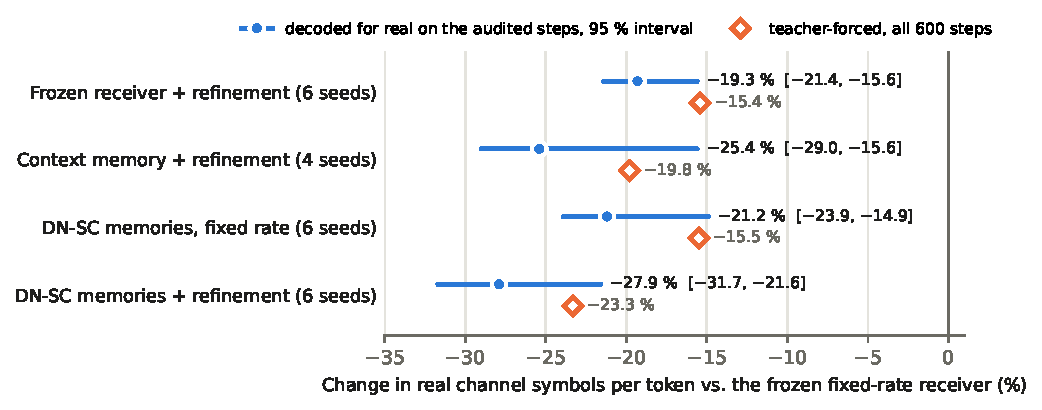
\includegraphics[width=0.92\linewidth]{figures/fig_primary_endpoint.pdf}
\caption{Change in real channel symbols per token for 90\,\% token accuracy against the frozen fixed-rate receiver, return-link signalling of refinement included. Dots: decoded for real on the audited steps, with 95\,\% paired bootstrap intervals; diamonds: teacher-forced on all 600 steps.}
\label{fig:primary}
\end{figure}

By the decision rule of Section~\ref{sec:setup-protocol}, the teacher-forced curves stand: on the audited steps, real decoding needs $+3.4$\,\% (context memory), $+3.6$\,\% (DN-SC) and $+5.0$\,\% (frozen receiver) more forward symbols at the target than the emulation. The frozen receiver sits at the limit of the rule, which is why both measurements are reported throughout. The real-decoding savings are larger than the teacher-forced ones because a fixed prefix suffers more from error propagation than the refinement policy does: decoded for real, the frozen fixed-rate receiver needs 10.37 symbols per token instead of 9.23. Figure~\ref{fig:operating} shows the pooled operating curves decoded for real. Refinement shifts the curve of the frozen receiver to the left above about 85\,\% accuracy; the memories of DN-SC raise the fixed-prefix curve at every rate, which leaves less to refinement.

\begin{figure}[t]
\centering
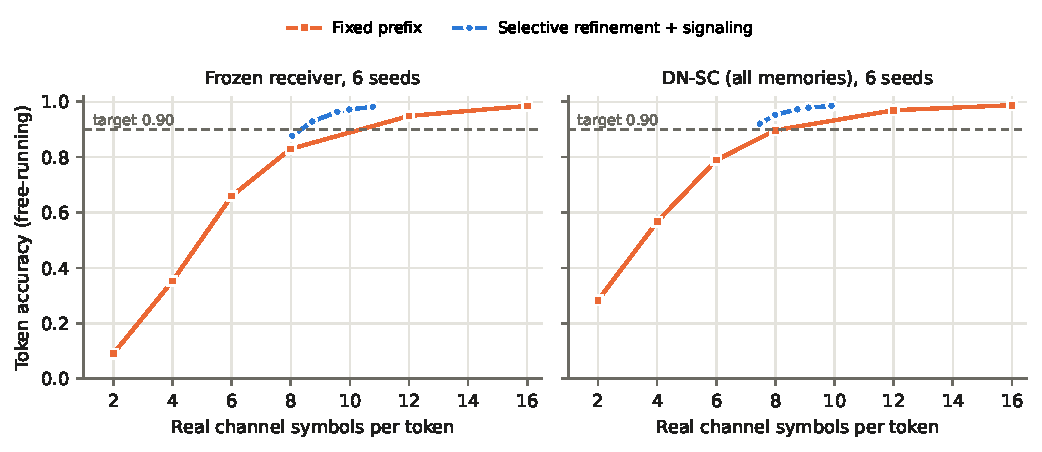
\includegraphics[width=\linewidth]{figures/fig_operating.pdf}
\caption{Operating curves decoded for real on the audited steps of the drift stream, pooled over six seeds (156 steps, 936 messages per receiver). Fixed prefix: all six prefix lengths. Selective refinement: thresholds $\tau = 0.5$ to $0.99$ from left to right, with the return-link signalling at its entropy added to the forward symbols.}
\label{fig:operating}
\end{figure}

\subsection{Where the saving comes from}
\label{sec:results-decomposition}

Receiver memories and selective refinement both contribute, and their contributions overlap (Table~\ref{tab:primary}). At a fixed rate, the memories of DN-SC alone save 15.5\,\% teacher-forced (21.2\,\% decoded for real), with no return-link signalling. Refinement alone saves the frozen receiver 15.4\,\% (19.3\,\% decoded for real). On top of the memories, refinement adds a further 9.3\,\% teacher-forced and 8.4\,\% decoded for real (95\,\% CI 3.9--18.3\,\%): the better the prior, the less uncertainty is left for refinement to resolve. Table~\ref{tab:decomposition} shows the mechanism. The prior cross-entropy, which measures what the receiver knows about a token before any symbol arrives, falls from 6.79 bits per token for the frozen receiver to 5.61 with the context memory and 5.23 with all memories. On the four seeds shared by all three receivers, the context memory accounts for 76\,\% of that reduction. The shipped memories lower the prior by a further 0.37 bits per token and the selective cost at $\tau = 0.9$ by 0.12 symbols per token; both intervals exclude zero, but with four seeds the seed-level test cannot go below $p = 0.125$. The signalling is light: at the operating threshold the requests cost 1.39 bits per token at the entropy (1.52 as a bitmap) over 2.84 rounds per message for DN-SC, against 1.62 bits and 3.07 rounds for the frozen receiver.

\begin{table}[t]
\centering
\caption{Mechanism of the saving on the drift stream (teacher-forced, all 600 steps). Prior cross-entropy: mean $\pm$ SD over seeds; differences to DN-SC are paired per step, with 95\,\% block-bootstrap intervals. Requests and rounds at the operating threshold $\tau = 0.9$.}
\label{tab:decomposition}
\footnotesize\setlength{\tabcolsep}{3.6pt}
\begin{tabular}{@{}lcccccc@{}}
\toprule
Receiver & Seeds & \makecell{Prior cross-entropy\\(bits/token)} & \makecell{Difference to DN-SC\\{[95\,\% CI]}} & \makecell{Requests (bits/token)\\entropy / bitmap} & \makecell{Rounds per\\message} & \makecell{Synchronisation\\(kbit/step)} \\
\midrule
Frozen & 6 & $6.79\pm0.04$ & $+1.56$ [$+1.41$, $+1.72$] & 1.62 / 1.69 & 3.07 & 0 \\
Context memory & 4 & $5.61\pm0.02$ & $+0.37$ [$+0.32$, $+0.41$] & 1.40 / 1.53 & 2.81 & 0 \\
DN-SC & 6 & $5.23\pm0.02$ & --- & 1.39 / 1.52 & 2.84 & 24.23 \\
\bottomrule
\end{tabular}
\end{table}

Figure~\ref{fig:prior_stream} shows the prior along the stream. Within AG News the three receivers differ by less than one bit per token. On the first switch to TeleQnA the frozen prior rises, while the context memory and DN-SC fall to about 5 bits per token within one topic period; a TeleQnA document---question, explanation and answer---repeats much of its own vocabulary, which the context makes available to the prior. The shipped memories add their gain mainly in TeleQnA, and more on its second visit, which is consistent with the recall of the adapter slot learned during the first visit (3.3 slot switches per run on average).

\begin{figure}[t]
\centering
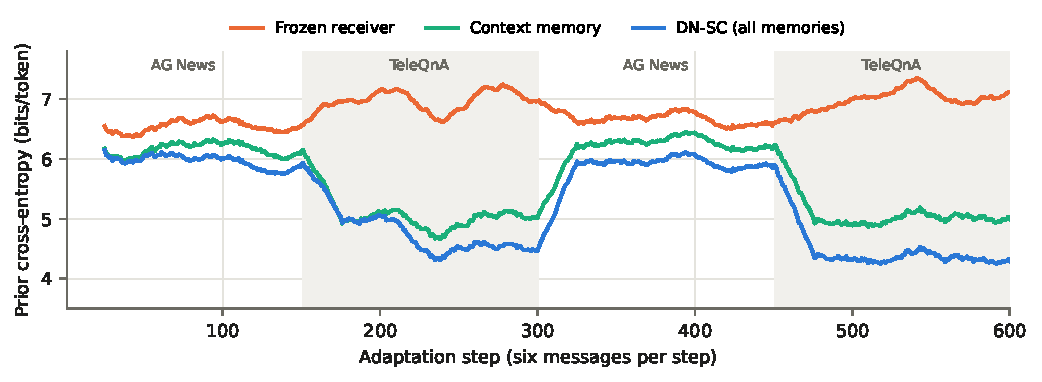
\includegraphics[width=\linewidth]{figures/fig_prior_stream.pdf}
\caption{Prior cross-entropy along the hierarchical drift stream (25-step moving average, mean over the four seeds shared by the three receivers). Shaded: TeleQnA regimes.}
\label{fig:prior_stream}
\end{figure}

\subsection{Component analysis}
\label{sec:results-ablation}

Table~\ref{tab:ablation} reports the components of the memories from the pilot runs, made with an earlier version of the code on a T4 GPU (greedy decoder, first round of 2 symbols, one to three seeds per receiver). They are exploratory, and only the prior cross-entropy is reported, because it does not depend on the decoder of refinement except through the context. The context memory is indispensable: DN-SC without it is 1.14 bits per token worse. Adapter slots help: a single adapter that is dragged between the domains costs 0.10 bits per token. Shipping both gradient levels at one period with the same synchronisation budget and one adapter (single-rate) costs 0.11 bits, and adding elastic weight consolidation \cite{kirkpatrick2017} to it does not help (0.12). The two separate shipping periods, however, are not shown to matter: with slots and context kept and both levels shipped at one period, the difference is 0.02 bits per token, within the equivalence margin of $\pm0.05$, on one seed. Shipping after every step costs 49 times the air time of DN-SC and is equivalent to it within the same margin. On this stream, the gain of the shipped memories therefore comes from the adapter slots and from shipping rarely, not from separating the timescales of the two shipped levels.

\begin{table}[t]
\centering
\caption{Component analysis (pilot runs, exploratory): prior cross-entropy on the drift stream, mean $\pm$ SD over seeds, paired per-step difference to DN-SC with 95\,\% block-bootstrap interval, equivalence within $\pm0.05$ bits per token by two one-sided tests (90\,\% interval), and measured synchronisation.}
\label{tab:ablation}
\footnotesize
\begin{tabular}{@{}lccccc@{}}
\toprule
Receiver & Seeds & \makecell{Prior cross-entropy\\(bits/token)} & \makecell{Difference to DN-SC\\{[95\,\% CI]}} & \makecell{Equivalent\\($\pm0.05$)} & \makecell{Synchronisation\\(kbit/step)} \\
\midrule
Frozen & 3 & $6.793\pm0.044$ & $+1.538$ [$+1.315$, $+1.760$] & no & 0 \\
DN-SC without context & 1 & 6.435 & $+1.145$ [$+0.829$, $+1.444$] & no & 24.23 \\
Context memory & 3 & $5.628\pm0.023$ & $+0.373$ [$+0.322$, $+0.420$] & no & 0 \\
Single rate, one adapter & 3 & $5.363\pm0.024$ & $+0.107$ [$+0.076$, $+0.143$] & no & 23.73 \\
Single rate + EWC & 1 & 5.414 & $+0.123$ [$+0.073$, $+0.183$] & no & 23.73 \\
DN-SC without slots & 3 & $5.352\pm0.024$ & $+0.096$ [$+0.064$, $+0.135$] & no & 24.23 \\
DN-SC, one shipping period & 1 & 5.312 & $+0.022$ [$+0.013$, $+0.032$] & yes & 29.63 \\
\textbf{DN-SC} & 3 & $\mathbf{5.256\pm0.031}$ & --- & --- & 24.23 \\
Shipping after every step & 3 & $5.250\pm0.031$ & $-0.006$ [$-0.031$, $+0.020$] & yes & 1185.80 \\
\bottomrule
\end{tabular}
\end{table}

\subsection{When shipping adaptation pays}
\label{sec:results-crossover}

Shipping the updates is not free. DN-SC ships 24.23\,kbit per adaptation step; at the capacity of 10\,dB this occupies about 14{,}000 real channel symbols, roughly 110 times the payload of one message at the target accuracy (about 127 symbols). Figure~\ref{fig:netrate} shows the net semantic rate~(\ref{eq:netrate}) of DN-SC relative to three references, on the four seeds shared by all receivers, with the signalling of refinement included. Against the frozen fixed-rate receiver, shipping pays when one update serves more than about 400 messages, and the saving approaches 21.5\,\% for large traffic. Against the frozen receiver with refinement, the crossover is about 1250 messages (asymptote 8.1\,\%), and against the context memory with refinement, which costs no synchronisation, it is about 6100 messages, with an asymptotic saving of only 1.8\,\%. In the stream itself an update serves six messages. For a single link, the context memory with selective refinement is therefore the economical configuration; shipped adaptation pays where one update serves many messages, such as the users of a cell or a multicast group that share a domain.

\begin{figure}[t]
\centering
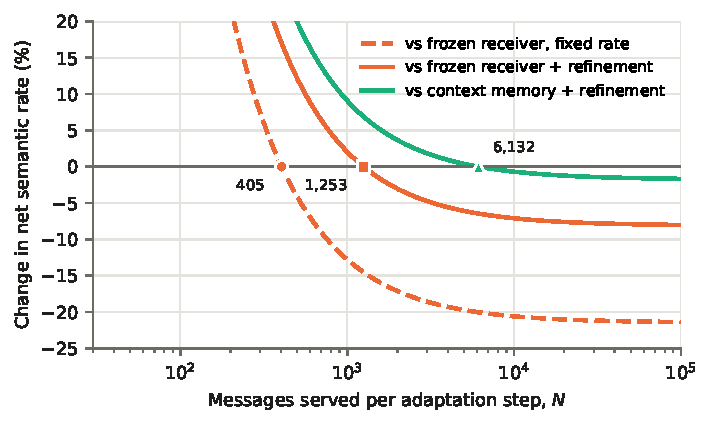
\includegraphics[width=0.72\linewidth]{figures/fig_netrate.pdf}
\caption{Change in the net semantic rate of DN-SC, synchronisation included, relative to three references, against the number of messages one adaptation step serves (four seeds shared by all receivers; return-link signalling at the entropy; synchronisation charged at the capacity of 10\,dB). Markers and numbers: crossover traffic $N^\star$.}
\label{fig:netrate}
\end{figure}

\subsection{Complexity}
\label{sec:results-complexity}

The receiver adds three small sets of parameters to the frozen GPT-2 model (124,439,808 parameters): the codebook (213,248, trained once), the medium memory (771 values in the bit ledger, of which 770 are active in this configuration) and one adapter slot (147,456 per slot). On a T4 GPU with one CPU thread, decoding one message of 19 tokens with the language prior took about 195\,ms with greedy decoding, against 3.4\,ms without a prior; the language model dominates the cost. A complete 600-step run of DN-SC, including 26 audited steps decoded for real at five thresholds and six prefix lengths with beam width 4, took 1.45--1.63\,h on one thread of the Linux CPU, against 0.99--1.11\,h for the frozen receiver. The transmitter must run the language model to learn the receiver's prior, so adaptation costs transmitter computation in addition to air time.

\subsection{Discussion and limitations}
\label{sec:results-discussion}

\emph{What the results support.} Every claim in this section is read from result files that the code writes and that are public (Data Availability Statement), on a protocol that was fixed before the confirmatory runs and that allowed the results to go against the method. Three findings are robust: a language prior with selective refinement saves channel symbols against a fixed-rate receiver with the same decoder, signalling included; the free context memory supplies most of what the memories gain; and shipped adaptation pays only above a traffic volume that a single link does not reach. The time-nesting of the shipped memories is the weakest component: the pilot ablation does not show that separating their periods matters, and its measured benefit over the context memory is small.

\emph{Position against separate source--channel coding.} An idealised separate design that compresses each message by arithmetic coding with the same GPT-2 model and sends it with a finite-block-length channel code in the normal approximation \cite{polyanskiy2010} delivers 42\,\% of the base-corpus messages intact at 4 symbols per token and 96.5\,\% at 6 (AWGN, 10\,dB, known SNR). This is a bound, not a system, but it shows that the uncoded token-level codec does not beat separation at a fixed rate and a known SNR (85.7\,\% token accuracy at 6 symbols, Table~\ref{tab:base}). What DN-SC offers instead is graceful degradation without a cliff, a rate that the receiver adapts per token, and an explicit account of what keeping the knowledge aligned costs.

\emph{Limitations.}
(i) One language model (GPT-2 with 124 million parameters) and one codebook were used, on CPUs; larger models will give stronger priors, at a higher cost of computation and of every adapter shipment.
(ii) Six seeds give $p = 0.031$ for each comparison of a refinement receiver with the frozen fixed-rate receiver; Holm-adjusted over the three receivers, the smallest value is 0.094. The context memory receiver has four seeds, and its test cannot go below 0.125.
(iii) The channel is simulated (AWGN on the stream), with perfect channel state information and a known message length; signalling and synchronisation are charged at capacity and assumed error-free, and the delay of several rounds is counted but not modelled.
(iv) On the stream, refinement and the receiver's context are emulated teacher-forced on every step and verified by real decoding on one step in 23; the context is built from the emulated decisions.
(v) The component analysis comes from pilot runs of an earlier code version with one to three seeds; it was not repeated with the final decoder.
(vi) The stream is text only and designed with hierarchical drift; a stream with naturally occurring drift was not repeated with the final decoder.
(vii) Adapter slots are allocated greedily and never recycled, and a token is sent as an uncoded real vector without an outer channel code.
